\begin{question}
\noindent Triangle $A$ is translated to triangle $B$, as shown on the grid below.

\begin{center}
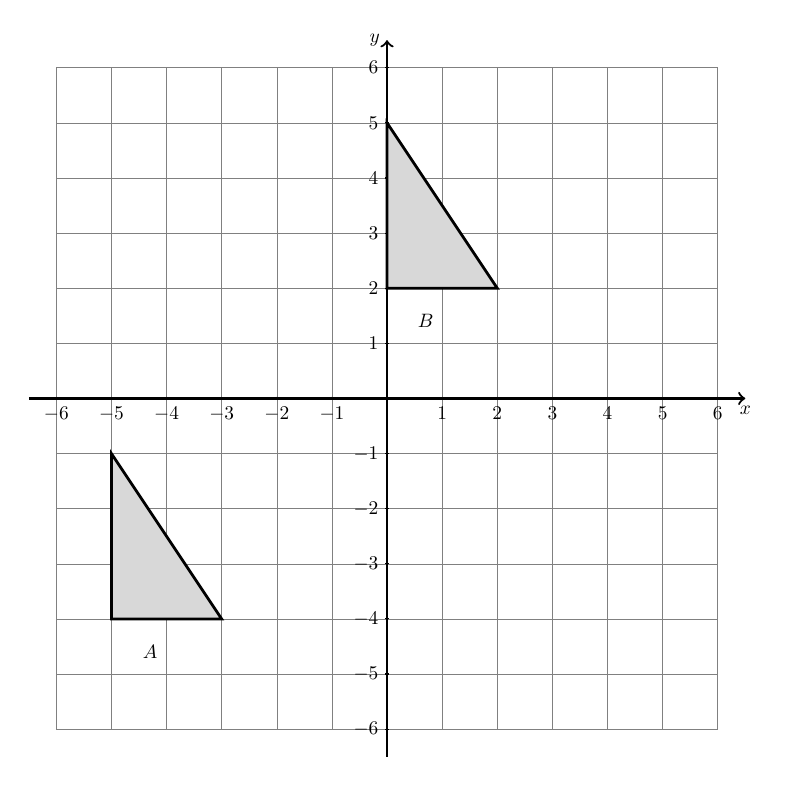
\begin{tikzpicture}[scale=0.7, transform shape]
    % Define axis scale
    \def\axisLimit{6}

    \definecolor{borderColour}{HTML}{000000}
    \definecolor{fillColour}{HTML}{D8D8D8}

    % Draw grid
    \draw[step=1cm,gray,very thin] (-\axisLimit,-\axisLimit) grid (\axisLimit,\axisLimit);

    % Draw axes
    \draw[thick,->] (-\axisLimit-0.5,0) -- (\axisLimit+0.5,0) node[anchor=north] {$x$};
    \draw[thick,->] (0,-\axisLimit-0.5) -- (0,\axisLimit+0.5) node[anchor=east] {$y$};

    % Label x-axis and y-axis
    \foreach \x in {-6,-5,...,-1,1,2,...,6}
        \draw (\x cm,1pt) -- (\x cm,-1pt) node[anchor=north] {$\x$};
    \foreach \y in {-6,-5,...,-1,1,2,...,6}
        \draw (1pt,\y cm) -- (-1pt,\y cm) node[anchor=east] {$\y$};

    % Define coordinates for triangle A
    \coordinate (P1) at (-5,-4);
    \coordinate (P2) at (-5,-1);
    \coordinate (P3) at (-3,-4);

    % Draw triangle A
    \filldraw[fill=fillColour, draw=borderColour, line width=1pt] (P1) -- (P2) -- (P3) -- cycle;
    \node at (-4.3,-4.6) {$A$};

    % Define coordinates for triangle B (translated by (5,6))
    \coordinate (Q1) at (0,2);
    \coordinate (Q2) at (0,5);
    \coordinate (Q3) at (2,2);

    % Draw triangle B
    \filldraw[fill=fillColour, draw=borderColour, line width=1pt] (Q1) -- (Q2) -- (Q3) -- cycle;
    \node at (0.7,1.4) {$B$};

\end{tikzpicture}
\end{center}

\noindent Describe fully the translation that maps triangle $A$ onto triangle $B$.

\vspace{4cm}

\begin{flushright}
    \answerplain{2}
\end{flushright}
\end{question}